\documentclass[tikz,border=4pt]{standalone}
\usepackage{amsmath}
\usepackage{tikz}
\usetikzlibrary{arrows.meta,decorations.markings}
\begin{document}
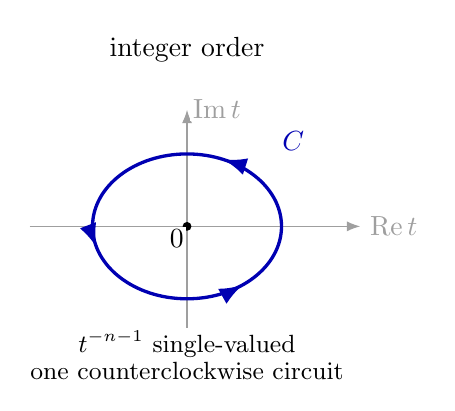
\begin{tikzpicture}[>=Latex,scale=1.0]
  \tikzset{
    axis/.style={->,gray!75},
    contour/.style={very thick,blue!70!black},
    branch/.style={very thick,orange!80!black},
    tag/.style={fill=white,inner sep=1pt}
  }

  \begin{scope}
    \node at (0,2.25) {integer order};
    \draw[axis] (-2.0,0) -- (2.2,0) node[right] {$\operatorname{Re}t$};
    \draw[axis] (0,-1.85) -- (0,1.48);
    \node[tag,text=gray!75] at (0.38,1.49) {$\operatorname{Im}t$};
    \fill (0,0) circle (1.6pt) node[tag,below left] {$0$};
    \draw[contour,postaction={decorate},
      decoration={markings,mark=at position .18 with {\arrow{Latex}},
      mark=at position .54 with {\arrow{Latex}},
      mark=at position .86 with {\arrow{Latex}}}]
      (0,0) ellipse (1.2 and 0.92);
    \node[tag,text=blue!70!black] at (1.35,1.08) {$C$};
    \node[align=center,tag,font=\small] at (0,-1.64)
      {$t^{-n-1}$ single-valued\\[-1pt]one counterclockwise circuit};
  \end{scope}


\end{tikzpicture}
\end{document}
